\documentclass[11pt,letterpaper]{article}
\usepackage[lmargin=1in,rmargin=1in,bmargin=1in,tmargin=1in]{geometry}
\usepackage{checkins}


% -------------------
% Content
% -------------------
\begin{document}
\thispagestyle{title}

% 08/22
\checkin{08/22} Let $f(x)$ be a relation with $f(2)= 7$ and $f(-3)= 7$. Because $f(2)$ and $f(-3)$ are both $7$, $f$ cannot be a function. \pspace

\sol The statement is \textit{false}. A relation is a function if there is only one possible output for a given input, i.e. given an input, one knows with certainty what the output is. We know that $f(2)= 7$ and $f(-3)= 7$; that is, given the inputs of $x= 2$ or $x= -3$, we know the output. The fact that the outputs are the same is irrelevant. There are many functions with the property that $f(2)= 7$ and $f(-3)= 7$. For instance, there must be a linear function through these two points, i.e. $y= 7$. An example of a quadratic function through these points is $y= \frac{7x(x + 1)}{6}$. \pvspace{1.3cm}



% 08/27
\checkin{08/27} If $S(t)= 0.008t + 57.81$ represents the stock price for a company $t$ minutes after opening, then the rate of change of the stock value is $0.008$, i.e. the stock is gaining $\$0.008$ per minute in value, and the opening price of the stock was $\$57.81$. \pspace

\sol The statement is \textit{false}. The stock price at opening would be the stock price at $t= 0$. But $S(0)= 0.008(0) + 57.81= 57.81$. Therefore, the opening stock price was \$57.81. Observe that $S(t)$ is a linear function, i.e. a function of the form $y= mx + b$ with $y= S$, $x= t$, $m= 0.008$, and $b= 57.81$. We know the rate of change of a linear function is its slope. But then the rate of change of $S(t)$ is $m= 0.008$, i.e. there is an increase of \$0.008 per minute in the value of the stock. \pvspace{1.3cm}



% 08/29
\checkin{08/29} If the production cost of a certain item is constant, then the cost to produce $q$~items, $C(q)$ is linear. Furthermore, the slope of $C(q)$ is the marginal cost and $C(0)$ is the fixed cost. \pspace

\sol The statement is \textit{true}. If the cost of production for the item is constant, then the production cost has a constant rate of change. But then the cost function to produce $q$ items, $C(q)$, must be linear. We know the marginal cost for a linear cost function is its slope. Furthermore, $C(0)$ is the fixed costs. But the $y$-intercept of $C(q)$ is precisely $C(0)$. \pvspace{1.3cm}



% 09/03
\checkin{09/03} Let $f(x)= 17(0.93)^x$. Because $f(x)$ the form $Ab^x$ with $A= 17$ and $b= 0.93$, it is exponential. Furthermore, $A= 17$ represents the $y$-intercept of $17$, i.e. an initial value of $17$, and $b= 0.93$ can be interpreted as a 93\% decrease of the initial value of $17$ a total of $x$-times. \pspace

\sol The statement is \textit{false}. An exponential function is a function of the form $Ab^x$. Therefore, $f(x)= 17(0.93)^x$ is an exponential function with $A= 17$ and $b= 0.93$. We know that $A= 17$ is the $y$-intercept because $f(0)= 17(0.93)^0= 17(1)= 17$. We know that for any exponential function, we can interpret $b$ as a percentage increase/decrease. We know that $0 < b < 1$. Therefore, we know that $f(x)$ is exponentially decreasing. We have $b= 0.93= 1 - 0.07$. Therefore, we can interpret $f(x)$ as a 7\% decrease of the initial value of $17$ a total of $x$-times. \pvspace{1.3cm}



\newpage



% 09/05
\checkin{09/05} Because multiplication is commutative, $(f \circ g)(x)= (g \circ f)(x)$. \pspace

\sol The statement is \textit{false}. It is true that multiplication is commutative. However, $f \circ g$ does not denote multiplication but rather function composition. We know that $(f \circ g)(x)= f \big( g(x) \big)$. There is no need for $(f \circ g)(x)= (g \circ f)(x)$. Although it can happen, it is certainly (typically) false. For instance, if $f(x)= 0$ and $g(x)= 1$. Then $(f \circ g)(x)= f \big( g(x) \big)= f(1)= 0$ and $(g \circ f)(x)= g \big( f(x) \big)= g(0)= 1$. \pvspace{1.3cm}



% 09/19
\checkin{09/19} If $f(x)$ is a function which is twice differentiable and $f'(x) > 0$, then $f''(x) > 0$. \pspace

\sol The statement is \textit{false}. Recall that if $f'(x) > 0$, the function $f(x)$ is increasing at that $x$-value, and if $f'(x) < 0$, the function $f(x)$ is decreasing at that $x$-value. Furthermore, recall that if $f''(x) > 0$, the function $f(x)$ is concave up at that $x$-value, and if $f''(x) < 0$, the function $f(x)$ is concave down at that $x$-value. Therefore, the question is asking if a function is increasing, does it have to be concave up. This is certainly not the case. For instance, consider the function $f(x)$ shown below. 
	\[
	\fbox{
	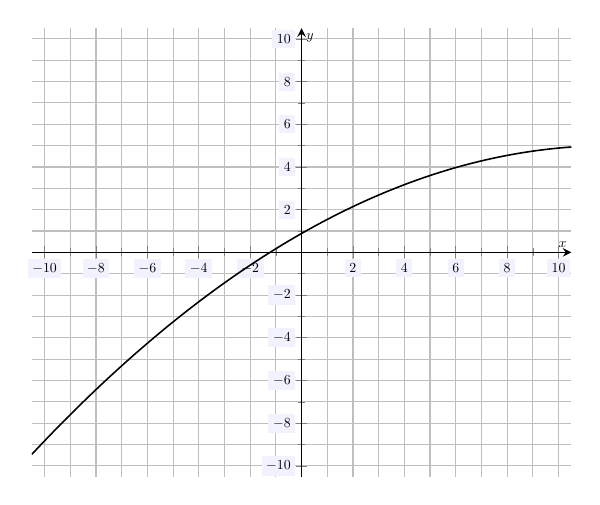
\begin{tikzpicture}[scale=1,every node/.style={scale=0.5}]
	\begin{axis}[
	grid=both,
	axis lines=middle,
	ticklabel style={fill=blue!5!white},
	xmin= -10.5, xmax=10.5,
	ymin= -10.5, ymax=10.5,
	xtick={-10,-8,-6,-4,-2,0,2,4,6,8,10},
	ytick={-10,-8,-6,-4,-2,0,2,4,6,8,10},
	minor tick = {-10,-9,...,10},
	xlabel=\(x\),ylabel=\(y\),
	]
	\addplot[line width= 0.02cm,samples=100,domain= -10.5:10.5] ({x},{5 - 1/35*(x - 12)^2});
	\end{axis}
	\end{tikzpicture}
	}
	\] 
This function is clearly everywhere increasing, so that $f'(x) > 0$. However, observe that the function is concave down, so that $f''(x) < 0$. The sign of $f'$ and $f''$ do indeed give you information about $f(x)$. However, the signs of $f$, $f'$, and $f''$ \textit{do not} need to be the same. \pvspace{1.3cm}



% 09/24
\checkin{09/24} If $C(q)$ is a cost function, then $C'(q)$ is the marginal cost. \pspace

\sol The statement is \textit{true}. In the case of linear cost functions, we knew that the marginal cost was the slope of the line, i.e. its derivative. For general cost functions, we define the marginal cost to be the derivative of the cost function. Generally, we know the marginal cost is the cost of producing the next item. We know that $C'(q):= \frac{dC}{dq}$. But then the cost of the next item should approximately be $\frac{dC}{dq} \big( (q+1) - q \big)= \frac{dC}{dq} \cdot 1= \frac{dC}{dq}$. That is, the cost of the next additional item is approximately $C'(q)$. \pvspace{1.3cm}



\newpage



% 09/26
\checkin{09/26} $\dfrac{d}{dx} (7x^3 - e^x + \log_2 x)= 21x^2 - e^x + \dfrac{1}{x \ln 2}$ \pspace

\sol The statement is \textit{true}. Recall that $\frac{d}{dx} \, x^n= nx^{n-1}$, $\frac{d}{dx}\, e^x= e^x$, and $\frac{d}{dx}\, \log_2 x= \frac{1}{x \ln 2}$. Therefore, we have\dots
	\[
	\dfrac{d}{dx} (7x^3 - e^x + \log_2 x)= (7 \cdot 3 x^2 - e^x + \dfrac{1}{x \ln 2})= 21x^2 - e^x + \dfrac{1}{x \ln 2}
	\] \pvspace{1.3cm}



% 10/03
\checkin{10/03} $\dfrac{d}{dx} \left(4x^2 - \dfrac{1}{x} \right)^5= 5 \left(8x - \dfrac{1}{x^2} \right)^4$ \pspace

\sol The statement is \textit{false}. Recall that the chain rule states that $\frac{d}{dx} f \big( g(x) \big)= f' \big( g(x) \big) \cdot g'(x)$. We have here $f(x)= x^5$ and $g(x)= 4x^2 - \frac{1}{x}$. We know that $f'(x)= 5x^4$ and $g'(x)= 8x + \frac{1}{x^2}$. Therefore, we have\dots
	\[
	\dfrac{d}{dx} \left(4x^2 - \dfrac{1}{x} \right)^5= 5 \left(4x^2 - \dfrac{1}{x} \right)^4 \cdot \left( 8x + \frac{1}{x^2} \right)
	\] \pvspace{1.3cm}



% 10/08
\checkin{10/08} Suppose that $f(1)= 5$, $f'(1)= 4$, and $f''(1)= -3$. Because $f'(1) > 0$, $f(x)$ is increasing at $x= 1$. Furthermore, because $f''(1) < 0$, $x= 1$ must be a local maxima for $f(x)$. \pspace

\sol The statement is \textit{false}. It is true that if $f'(a) > 0$, then $f(x)$ is increasing at $x= a$. Therefore, because $f'(1) > 0$, $f(x)$ is increasing at $x= 1$. We know that if $f''(a) < 0$ \textit{and} $f'(a)= 0$, then $f(x)$ has a local maxima at $x= a$---this is the second derivative test. Though $f''(1) < 0$, we know $f'(1) \neq 0$ because $f'(1) > 0$. Therefore, $x= 1$ need not be a local maxima. For instance, the function below has $f(1)= 5$, $f'(1)= 4$, and $f''(1)= -3$ but $x= 1$ is not a local maxima. 
	\[
	\fbox{
	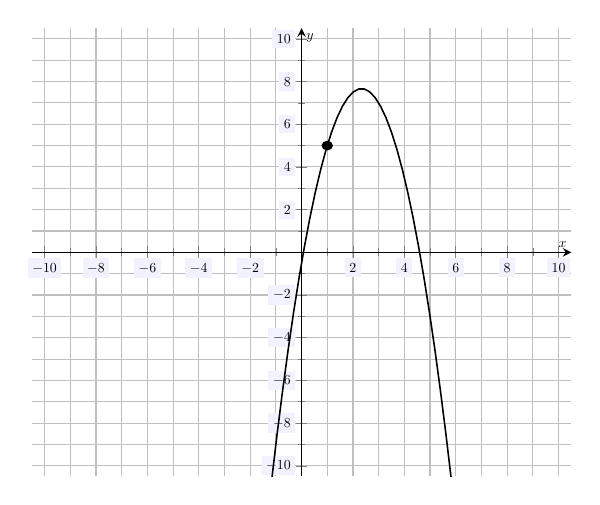
\begin{tikzpicture}[scale=1,every node/.style={scale=0.5}]
	\begin{axis}[
	grid=both,
	axis lines=middle,
	ticklabel style={fill=blue!5!white},
	xmin= -10.5, xmax=10.5,
	ymin= -10.5, ymax=10.5,
	xtick={-10,-8,-6,-4,-2,0,2,4,6,8,10},
	ytick={-10,-8,-6,-4,-2,0,2,4,6,8,10},
	minor tick = {-10,-9,...,10},
	xlabel=\(x\),ylabel=\(y\),
	]
	\addplot[line width= 0.02cm,samples=100,domain= -10.5:10.5] ({x},{-3/2*x^2 + 7*x - 1/2});
	\draw[fill=black] (1,5) circle (0.2);
	\end{axis}
	\end{tikzpicture}
	}
	\] 



\newpage



% 10/10
\checkin{10/10} Suppose that $f(-2)= 10$ and $f'(-2)= 0$. If $f'$ changes sign from positive to negative across $x= -2$, then $f(x)$ has a local maximum at $x= -2$. \pspace

\sol The statement is \textit{true}. This is the first derivative test. We know that if $f'(a)= 0$ and $f'(x)$ changes sign from positive to negative across $x= a$, then $x= a$ is a local maximum. 
	\[
	\begin{tikzpicture}
	\draw[line width=0.03cm,<->] (-3,0) -- (3,0);
	\draw[line width=0.03cm] (0,-0.1) -- (0,0.1);
	\node at (-0.12,-0.35) {$-2$};
	\node at (-1.3,0.3) {$+$};
	\node at (1.3,0.3) {$-$};
	\draw[line width=0.02cm] (-0.3,0.3) -- (-0.1,0.6) -- (0.1,0.6) -- (0.3,0.3);
	\end{tikzpicture}
	\]

























\end{document}